\documentclass{article}%
\usepackage[T1]{fontenc}%
\usepackage[utf8]{inputenc}%
\usepackage{lmodern}%
\usepackage{textcomp}%
\usepackage{lastpage}%
\usepackage[head=40pt,margin=0.5in,bottom=0.6in]{geometry}%
\usepackage{graphicx}%
%
\title{\textbf{Gremios consignaron documento en la Inspectoría del Trabajo para exigir mejoras salariales}}%
\author{SHARON BRITO}%
\date{05/10/2018}%
%
\begin{document}%
\normalsize%
\maketitle%
\textbf{URL: }%
http://www.eluniversal.com/politica/22442/diversos{-}gremios{-}entregaron{-}documento{-}a{-}inspectoria{-}del{-}trabajo\newline%
%
\textbf{Periodico: }%
EU, %
ID: %
22442, %
Seccion: %
politica\newline%
%
\textbf{Palabras Claves: }%
NO\_TIENE\newline%
%
\textbf{Derecho: }%
2.3, %
Otros Derechos: %
, %
Sub Derechos: %
2.3.4\newline%
%
\textbf{EP: }%
SI\newline%
\newline%
%
\textbf{\textit{El texto fue dirigido al ministro Eduardo Piñate. En el interior del país también se produjeron movilizaciones similares hacia las dependencias regionales de la Inspectoría del Trabajo}}%
\newline%
\newline%
%
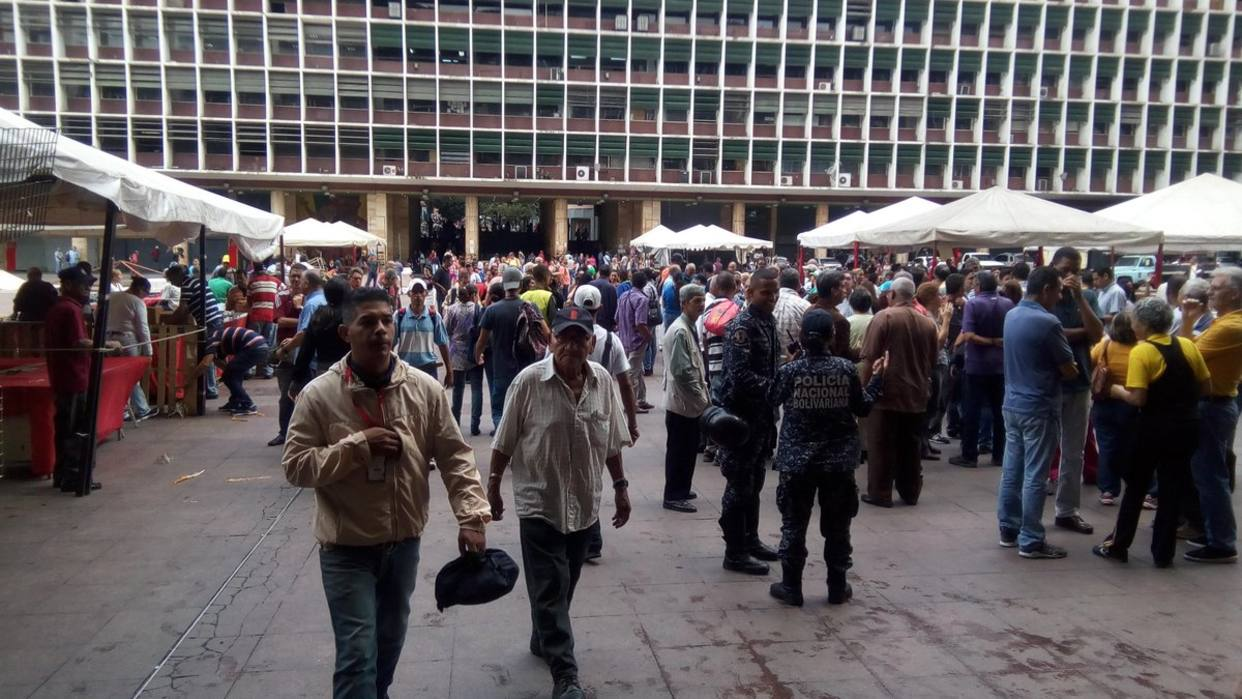
\includegraphics[width=300px]{56.jpg}%
\newline%
%
Caracas.{-} Representantes de trabajadores de diversos gremios que hacen vida en el país se dirigieron este viernes a la Inspectoría del Trabajo {-}luego de realizar una concentración en Plaza Caracas{-} para consignar un documento en demanda de mejoras salariales.%
\newline%
%
El documento fue dirigido al titular de la cartera de Trabajo, Eduardo Piñate, quien no atendió la recepción sino que fue recibida por el presidente del sindicato de ese ministerio.~En la concentración, realizada la mañana de hoy en Plaza Caracas, había representantes del sector educativo, de la salud, dirigentes estudiantiles, jubilados y pensionados de diferentes estatales y miembros de la sociedad civil.En estados como Bolívar, Mérida, Falcón, Guárico, Apure, Aragua, Miranda y Táchira distintos trabajadores y sindicatos también protestaron y se dirigieron a las respectivas Inspectorías del Trabajo de esas entidades para exigir reivindicaciones salariales.%
\newline%
%
Enfermeras exigen dotación de insumos en los hospitales%
\newline%
%
Por otra parte, la presidenta del Colegio de Enfermeras del Distrito Capital, Ana Rosario Contreras, exigió al Ejecutivo nacional "respetar al artículo 91 de la Constitución" al mencionar que el "Gobierno debe garantizar un salario mínimo para que podamos tener calidad de vida y no estar en pobreza extrema, como es la cruda realidad de los venezolanos”.%
\newline%
%
En declaraciones a Unión Radio, Contreras pidió al Gobierno la dotación de insumos en los hospitales. "Llego el momento en que los trabajadores venezolanos digamos basta al ensayo y error que se está haciendo con nuestras relaciones laborales; exigimos la dotación de nuestros hospitales para poder cumplir con nuestra buenas prácticas profesionales".%
\newline%
%
\end{document}